\section{ХОД РАБОТЫ}

\subsection{Задание}

Необходимо решить задачу повышения производительности труда не ниже заданного уровня
при соблюдении установленного лимита капитальных вложений. В соответствии с выбранным вариантом
имеем следующие исходные данные:

\begin{itemize}
  \item планируемый прирост производительности труда за год ---~11,0~\%;
  \item сумма выделенных капитальных вложений ---~700~млн~ден.~ед.;
  \item общая численность промышленно-производственного персонала ---~2520~чел.
\end{itemize}

\subsection{Решение задачи}

\paragraph{Подбор мероприятий.}

Необходимо подобрать мероприятия, обеспечивающие плановый прирост производительности
труда, оставаясь в пределах выделенного лимита капитальных вложений.

Данные о возможных мероприятиях представлены в таблицах 1.2-1.4 методического пособия.
Мероприятия, находящиеся в таблице 1.2 будем называть \textit{мероприятиями первой группы}, 
таблицах 1.3 и 1.4 --- \textit{мероприятиями второй и третьей} группы соответственно.

Для облегчения процесса выбора мероприятий выполним следующие операции:

\begin{enumerate}
  \item Для каждого мероприятия рассчитаем <<эффективность применения>>,
    как годовое повышение производительности труда, разделенное на капитальные вложения.
  \item Выполним сортировку мероприятия по <<эффективности применения>> в рамках каждой
    группы мероприятий.
\end{enumerate}

На рисунках~\ref{fig:tabl12}~--~\ref{fig:tabl14} представлены результаты проделанных операций.

\begin{figure}[htbp]
  \centering
  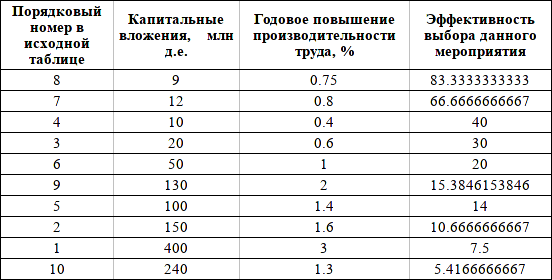
\includegraphics[width=0.8\linewidth]{img/tabl12}
  \caption{Результат обработки первой группы мероприятий}\label{fig:tabl12}
\end{figure}

\begin{figure}[htbp]
  \centering
  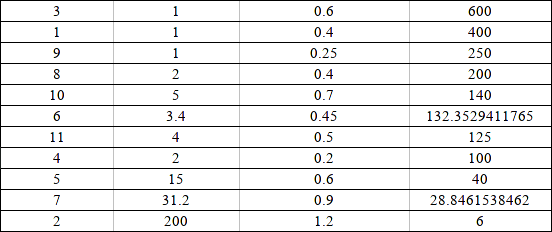
\includegraphics[width=0.8\linewidth]{img/tabl13}
  \caption{Результат обработки второй группы мероприятий}\label{fig:tabl13}
\end{figure}

\begin{figure}[htbp]
  \centering
  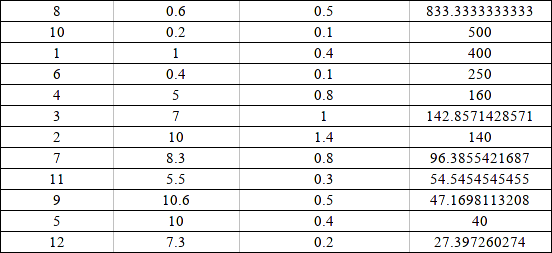
\includegraphics[width=0.8\linewidth]{img/tabl14}
  \caption{Результат обработки третьей группы мероприятий}\label{fig:tabl14}
\end{figure}

\newpage

Далее будем выбирать мероприятия с высокой <<эффективностью>> --- таким образом,
чтобы планируемый прирост производительности труда составил не менее 11\%.
Список выбранных мероприятий представлен в таблице~\ref{tbl:solution}.

\begin{table}[htbp]
  \caption{Выбранные мероприятия\label{tbl:solution}}
  \centering
    \begin{tabular}{| m{7.5cm} | m{3cm} | m{4.5cm} |}
      \hline
      Группа мероприятий / порядковый номер мероприятия &
      Капитальные \newline вложения, млн~ден.~ед. &
      Повышение \newline производительности труда, \% \\ \hline

      1/2 & 150 & 1{,}6 \\ \hline
      1/6 & 50 & 1 \\ \hline
      1/9 & 130 & 2 \\ \hline
      1/5 & 100 & 1{,}4 \\ \hline
      Итого по первой группе: & \textbf{430} & \textbf{6} \\ \hline

      2/3 & 1 & 0{,}6 \\ \hline
      2/4 & 2 & 0{,}2 \\ \hline
      2/8 & 1 & 0{,}4 \\ \hline
      2/9 & 1 & 0{,}25 \\ \hline
      2/10 & 5 & 0{,}7 \\ \hline
      2/11 & 4 & 0{,}5 \\ \hline
      Итого по второй группе: & \textbf{14} & \textbf{2{,}65} \\ \hline

      3/2 & 10 & 1{,}4 \\ \hline
      3/3 & 7 & 1 \\ \hline
      3/10 & 0{,}2 & 0{,}1 \\ \hline
      Итого по третьей группе: & \textbf{21{,}9} & \textbf{2{,}5} \\ \hline
      Итого: & 461{,}2 & 11{,}15 \\ \hline
    \end{tabular}
\end{table}

\paragraph{Расчет абсолютной экономии численности промышленно-производственного
 персонала} производится по формуле:
\begin{equation}
\% ~ \text{ПП} = \dfrac{\Delta\text{Ч}}{\text{Ч}_{\text{ПЛ}} - \Delta\text{Ч}} \cdot 100
\end{equation}

Выразим из этой формулы изменение численности персонала ($ \Delta\text{Ч} $).

Получим:
\begin{equation}
\Delta\text{Ч} = \dfrac{\% ~ \text{ПП} \cdot \text{Ч}_{\text{ПЛ}}}{100 + \% ~ \text{ПП}}
\end{equation}

Вычислим $ \Delta\text{Ч} $ по каждой группе мероприятий.
\begin{align*}
  \Delta\text{Ч}_{I} = \dfrac{6 \cdot 2520}{100 + 6} = 42 ~ \text{(чел.)} \\
  \Delta\text{Ч}_{II} = \dfrac{2.65 \cdot 2520}{100 + 2.65} = 63 ~ \text{(чел.)} \\
  \Delta\text{Ч}_{III} = \dfrac{2.5 \cdot 2520}{100 + 2.5} = 55 ~ \text{(чел.)}
\end{align*}

Итого за счет проведённых мероприятий абсолютная экономия численности
промышленно-производственного персонала составила \textbf{264 человека.}

\newpage
